\documentclass[10pt]{article}

%\usepackage{graphicx} % for \includegraphics

% amsmath package, useful for mathematical formulas
\usepackage{amsmath}
% amssymb package, useful for mathematical symbols
\usepackage{amssymb}

% cite package, to clean up citations in the main text. Do not remove.
\usepackage{cite}

\usepackage{hyperref}

% line numbers
\usepackage{lineno}

% ligatures disabled
\usepackage{microtype}
\DisableLigatures[f]{encoding = *, family = * }

% Text layout
\topmargin 0.0cm
\oddsidemargin 0.5cm
\evensidemargin 0.5cm
\textwidth 16cm
\textheight 21cm

% Bold the 'Figure #' in the caption and separate it with a period
% Captions will be left justified
\usepackage[labelfont=bf,labelsep=period,justification=raggedright]{caption}

% Use the PLoS provided BiBTeX style
\bibliographystyle{plos2009}

% Remove brackets from numbering in List of References
\makeatletter
\renewcommand{\@biblabel}[1]{\quad#1.}
\makeatother

% Leave date blank
\date{}

\pagestyle{myheadings}

\setcounter{secnumdepth}{0}

\begin{document}

\begin{flushleft}
{\large
\textbf{UniqTag: Content-derived unique and stable identifiers for gene annotation}
}
\\
Shaun Jackman$^{1,2,\ast}$,
Joerg Bohlmann$^{3}$,
\.{I}nan\c{c} Birol$^{1,4,\dagger}$
\\ \textbf{1} Genome Sciences Centre, British Columbia Cancer Agency, Vancouver, BC, Canada
\\ \textbf{2} Graduate Program in Bioinformatics, University of British Columbia, Vancouver, BC, Canada
\\ \textbf{3} Michael Smith Laboratories, University of British Columbia, Vancouver, BC, Canada
\\ \textbf{4} Department of Medical Genetics, University of British Columbia, Vancouver, BC, Canada
\\ $\ast$ E-mail: sjackman@bcgsc.ca, Twitter: @sjackman
\\ $\dagger$ E-mail: ibirol@bcgsc.ca
\end{flushleft}
\section{Abstract}\label{abstract}

When working on an ongoing genome sequencing and assembly project, it is
rather inconvenient when gene identifiers change from one build of the
assembly to the next. The gene labelling system described here, UniqTag,
addresses this common challenge. UniqTag assigns a unique identifier to
each gene that is a representative \emph{k}-mer, a string of length
\emph{k}, selected from the sequence of that gene. Unlike serial
numbers, these identifiers are stable between different assemblies and
annotations of the same data without requiring that previous annotations
be lifted over by sequence alignment. We assign UniqTag identifiers to
nine builds of the Ensembl human genome spanning seven years to
demonstrate this stability.

The implementation of UniqTag is available at
\url{https://github.com/sjackman/uniqtag}. Supplementary material and
code to reproduce it is available at
\url{https://github.com/sjackman/uniqtag-paper}.

\section{Introduction}\label{introduction}

The task of annotating the genes of a genome sequence often follows
genome assembly. These annotated genes are assigned unique identifiers
by which they can be referenced. Assembly and annotation is frequently
an iterative process, by refining the method or by the addition of more
sequencing data. These gene identifiers would ideally be stable from one
assembly and annotation to the next. The common practice is to use
serial numbers to identify genes that are annotated by software such as
MAKER {[}\href{http://dx.doi.org/10.1104/pp.113.230144}{1}{]}, which,
although certainly unique, are not stable between assemblies. A single
change in the assembly can result in a total renumbering of the
annotated genes.

One solution to stabilize identifiers is to assign them based on the
content of the gene sequence. A cryptographic hash function such as SHA
(Secure Hash Algorithm)
{[}\href{http://www.nist.gov/manuscript-publication-search.cfm?pub_id=910977}{2}{]}
derives a message digest from the sequence, such that two sequences with
the same content will have the same message digest, and two sequences
that differ will have different message digests. If a cryptographic hash
were used to identify a gene, the same gene in two assemblies with
identical content would be assigned identical identifiers. Yet, by
design a slight change in the sequence, such as a single-character
substitution, would result in a completely different digest.

Locality-sensitive hashing in contrast aims to assign items that are
similar to the same hash value. A hash function that assigns an
identical identifier to a sequence after a modification of that sequence
is desirable for labelling the genes of an ongoing genome annotation
project. One such locality-sensitive hash function, MinHash, was
employed to identify web pages with similar content
{[}\href{http://dx.doi.org/10.1109/SEQUEN.1997.666900}{3}{]} by
selecting a small representative set of words from a web page.

UniqTag is inspired by MinHash. It selects a single representative
\emph{k}-mer from a sequence to assign a stable identifier to a gene.
These identifiers are intended for systematic labelling of genes rather
than assigning biological gene names, as the latter are typically based
on biological function or homology to orthologous genes
{[}\href{http://dx.doi.org/10.1006/geno.2002.6748}{4}{]}. Assigning
UniqTag identifiers to the current assembly requires no knowledge of the
previous assemblies.

\section{Methods}\label{methods}

The UniqTag is defined mathematically as follows. Let \(\Sigma\) be an
alphabet, such as the twenty standard amino acids or the four
nucleotides. Let \(\Sigma^k\) be the set of all strings over \(\Sigma\)
of length \emph{k}. Let \emph{s} be a string over \(\Sigma\), such as
the peptide or nucleotide sequence of a gene. Let \(C(s)\) be the set of
all substrings of \emph{s}, and \(C_k(s)\) be the set of all
\emph{k}-mers of \emph{s}, that is, all substrings of \emph{s} with
length \emph{k}.

\[
C_k(s) = C(s) \cap \Sigma^k
\]

Let \emph{S} be a set of \emph{n} strings \(\{s_0, \dots, s_n\}\), such
as the peptide or nucleotide sequences of all the annotated genes of a
genome assembly. Let \(f(t, S)\) be the frequency in \emph{S} of a
\emph{k}-mer \emph{t}, defined as the number of strings in \emph{S} that
contain the \emph{k}-mer \emph{t}.

\[
f(t, S) = \left\vert \{ s \mid t \in C_k(s) \wedge s \in S \} \right\vert
\]

Let the function \(\min T\) define the lexicographically minimal string
of a set of strings \emph{T}. That is, if the strings of the set
\emph{T} were sorted alphabetically, \(\min T\) would refer to the first
string in the list.

Finally, \(u_k(s, S)\) is the UniqTag, the lexicographically minimal
\emph{k}-mer of those \emph{k}-mers of \emph{s} that are least frequent
in \emph{S}.

\[
u_k(s, S) = \min \mathop{\arg\,\min}\limits_{t \in C_k(s)} f(t, S)
\]

Typically, \(u_k(s, S)\) is the first \emph{k}-mer in an alphabetically
sorted list of the \emph{k}-mers of a gene that are unique to that gene.

A UniqTag can be generated from the nucleotide sequence of a gene or the
translated peptide sequence of a protein-coding gene. Using the peptide
sequence results in a UniqTag that is stable across synonymous changes
to the coding sequence as well as to changes in the untranslated regions
and introns of the gene. Since the amino acid alphabet is larger than
the nucleotide alphabet, fewer characters are required for a
\emph{k}-mer to be likely unique, resulting in an aesthetically pleasing
shorter identifier.

When two gene models have identical \emph{k}-mer compositions, they
would be assigned the same UniqTag. It is also possible that two genes
that have no unique \emph{k}-mer and similar \emph{k}-mer composition
are assigned the same UniqTag. In such cases, genes that have the same
UniqTag are distinguished by adding a numerical suffix to the UniqTag. A
UniqTag is formatted as a \emph{k}-mer followed by a hyphen and a
number, such as \emph{ARNDCEQGH-1}. For consistency of formatting the
suffix is always included, even when the \emph{k}-mer is unique and the
numerical suffix is \emph{-1}.

The UniqTag is designed to be stable but will change in the following
conditions: (1)~when the sequence at the locus of the UniqTag changes;
(2)~when a least-frequent \emph{k}-mer that is lexicographically smaller
than the previous UniqTag is created; (3)~when a duplicate \emph{k}-mer
is created elsewhere that results in the previous UniqTag no longer
being a least-frequent \emph{k}-mer.

The special cases of merging and splitting gene models are interesting.
Concatenating two gene models results in a gene whose UniqTag is the
minimum of the two previous UniqTags, unless the new UniqTag spans the
junction of the two sequences. Similarly when a gene model is split in
two, one gene is assigned a new UniqTag and the other retains the
previous UniqTag, unless the previous UniqTag spanned the junction.

Importantly and in contrast, unlike naming the genes after the genomic
contigs or scaffolds in which they are found, changing the names or the
order of the sequences in a genome assembly has no effect on the UniqTag
\emph{k}-mers of those genes.

\section{Results}\label{results}

To demonstrate the stability and utility of UniqTag, we assigned
identifiers to the genes of nine builds of the Ensembl human genome
{[}\href{http://dx.doi.org/10.1093/nar/gkt1196}{5}{]} (every fifth build
from 40 through 70 and build 74, all compared to build 75) spanning
seven years and two major genome assemblies (NCBI36 up to build 54 and
GRCh37 afterward). An identifier of nine amino acids (\(k=9\)) was
assigned to the first protein sequence, that with the smallest Ensembl
protein (ENSP) accession number, of each gene. The number of common
UniqTag identifiers between older builds from build 40 on and build 75
is shown in Figure~1. Also shown is the number of common gene and
protein identifiers (ENSG and ENSP accession numbers) between builds and
the number of genes with peptide sequences that are identical between
builds. Although less stable than the gene ID, the UniqTag is more
stable than the protein ID and the peptide sequence.

The stability of the UniqTag is insensitive to the size of the UniqTag
identifier for values of \emph{k} between 8 and 50 amino acids, shown in
Figure~2. The data for both figures are shown in supplementary Table~S1.

Sequences with the same peptide sequence are assigned the same UniqTag
\emph{k}-mer and disambiguated using the numerical suffix. Duplicate
UniqTag \emph{k}-mers due to hash collisions are rare, but can occur in
sequences that have no unique \emph{k}-mer, which is most likely with
short sequences. NCBI GRCh37 build 75 has 23,393 annotated genes, which
have 21,783 (93.1\%) distinct peptide sequences. Of these 21,783
distinct sequences, there are 54 (0.25\%) UniqTag collisions.

\section{Conclusions}\label{conclusions}

Whereas the gene and protein identifiers can, with effort, be lifted
over from older builds to the newest build, the UniqTag identifier can
be generated without any knowledge of previous assemblies, making it a
much simpler operation. The number of identical peptide sequences
between builds shows the stability that would be expected of using a
cryptographic hash value of the peptide sequence as the identifier. The
stability of the UniqTag is insensitive to the size of the UniqTag
\emph{k}-mer for a large range of \emph{k}.

\section{Acknowledgements}\label{acknowledgements}

The authors thank Nathaniel Street for his enthusiastic feedback, the
SMarTForests project and the organizers of the 2014 Conifer Genome
Summit that made our conversation possible.

\section{References}\label{references}

{[}1{]}~\href{http://dx.doi.org/10.1104/pp.113.230144}{Campbell MS, Law
MY, Holt C, Stein JC, Moghe GD, et al. (2014)} MAKER-P: a tool-kit for
the rapid creation, management, and quality control of plant genome
annotations. Plant Physiology 164: 513-524.
doi:10.1104/pp.113.230144\\{[}2{]}~\href{http://www.nist.gov/manuscript-publication-search.cfm?pub_id=910977}{Dang
QH (2012)} Secure Hash Standard (SHS). NIST FIPS 180:
1-35.\\{[}3{]}~\href{http://dx.doi.org/10.1109/SEQUEN.1997.666900}{Broder
AZ (1997)} On the resemblance and containment of documents. Compression
and Complexity of Sequences 1997 Proceedings: 21-29.
doi:10.1109/SEQUEN.1997.666900\\{[}4{]}~\href{http://dx.doi.org/10.1006/geno.2002.6748}{Wain
HM, Bruford EA, Lovering RC, Lush MJ, Wright MW, Povey S (2002)}
Guidelines for human gene nomenclature. Genomics 79: 464-470.
doi:10.1006/geno.2002.6748\\{[}5{]}~\href{http://dx.doi.org/10.1093/nar/gkt1196}{Flicek
P, Amode MR, Barrell D, Beal K, Billis K, et al. (2013)} Ensembl 2014.
Nucleic Acids Research 42: D749-D755. doi:10.1093/nar/gkt1196

\newpage

\section{Figure Legends}\label{figure-legends}

\begin{figure}[htbp]
\centering
%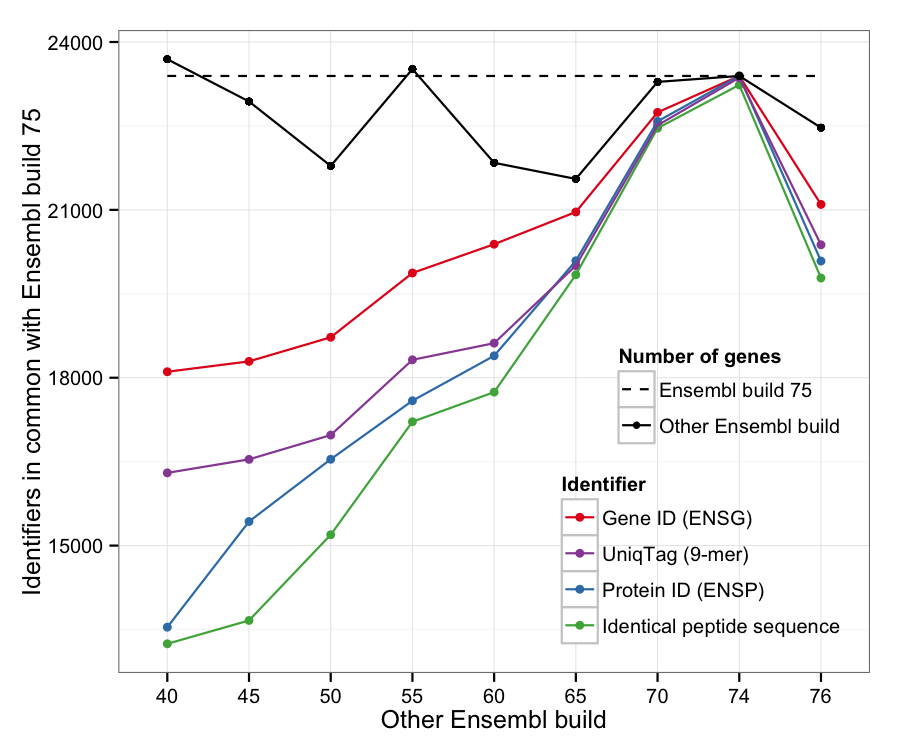
\includegraphics{figure/ensembl.png}
\caption{The number of common UniqTag identifiers between older builds
of the Ensembl human genome and build 75, the number of common gene and
protein identifiers between builds, and the number of genes with peptide
sequences that are identical between builds.}
\end{figure}

\begin{figure}[htbp]
\centering
%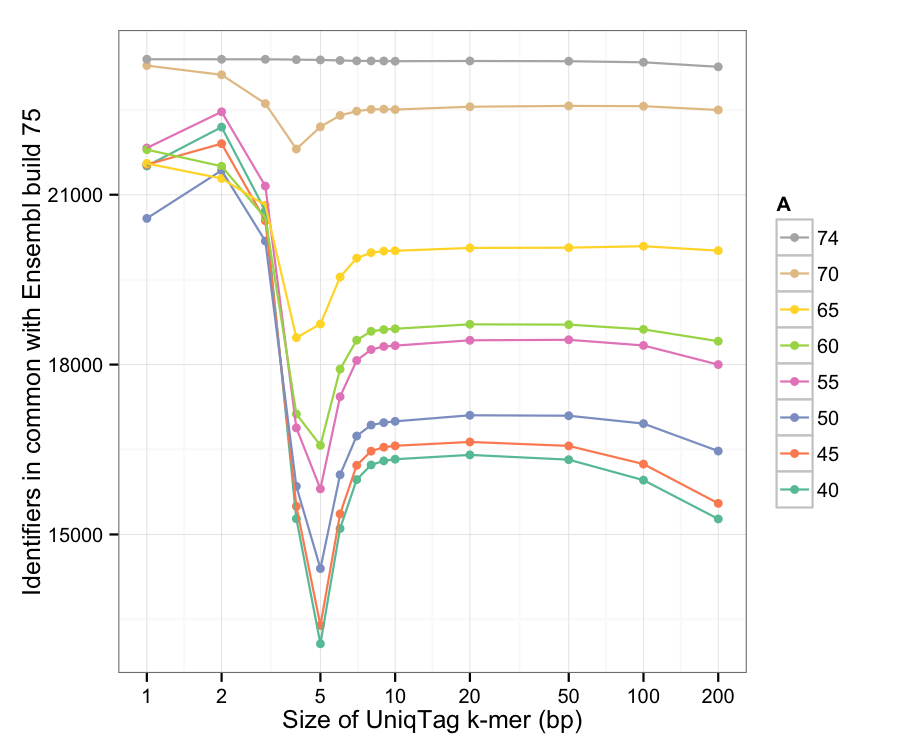
\includegraphics{figure/k.png}
\caption{The number of common UniqTag identifiers between older builds
of the Ensembl human genome and the current build 75 for different
values of \emph{k}.}
\end{figure}
\end{document}
